La suite de Syracuse s'exécute sur un nombre donné k qui consiste à diviser ce nombre par 2 si k est pair, ou le multiplier par 3 et lui ajouter 1 si celui-ci est impair ; on s'arrête quand on tombe sur 1. \\
On peut donc représenter cette suite de la manière suivante : \\ 

On a une suite $(U_n)$ avec $U_0 = k$ et 
$$
U_{n+1} = \left\{
    \begin{array}{ll}
        U_n/2 & \mbox{si } U_n \mbox{ pair} \\
        3*U_n + 1 & \mbox{si } U_n \mbox{ impair} \\
        1 \mbox{ fin} & \mbox{si } U_n = 1
    \end{array}
\right.
$$

Exemple sur 3 :
$$
U_0 = 3, U_1 = 10, U_2 = 5, U_3 = 16, U_4 = 8, U_5 = 4, U_6 = 2, U_7 = 1, fin.
$$

\subsubsection{Réalisation}
Pour la partie modèle, nous avons séparé en deux parties la suite de Syracuse. Dans la première, nous allons calculer la suite pour chaque nombre de 2 à la valeur que l'utilisateur donnera. Pendant le calcul de la suite sur un nombre on va compter le nombre d'itérations qu'il effectue dans la suite (en reprenant l'exemple sur 3, celui-ci effectue 7 itérations) et on stocke le nombre d'itérations dans une map (pour 3 on stocke la paire {3 => 7}). Si, pendant le calcul de la suite sur un nombre, on tombe sur un nombre dont le nombre d'itérations a déjà été calculé, on va additionner le nombre d'itérations que l'on a fait jusqu'ici avec le nombre d'itérations qu'on a stocké dans la map et cela correspondra au nombre d'itérations que le nombre effectue dans la suite de Syracuse. Dans la seconde partie, on va calculer la suite de Syracuse sur un nombre donné et on va stocker dans une liste chaque valeur obtenue (pour 3 la liste est [3, 10, 5, 16, 8, 4, 2, 1]).\\

Ensuite, pour la partie graphique, nous avons fait une première interface en Swing d'un graphique en barres correspondant à un nombre de 2 à n avec le nombre d'itérations dans la suite de Syracuse. On peut passer la souris sur le graphique et il indique en haut à gauche le nombre et son nombre d'itérations dans la suite (sur la Figure \ref{syra100}, on se trouve sur 97 qui fait 118 itérations dans la suite de Syracuse).

\begin{figure}[H]
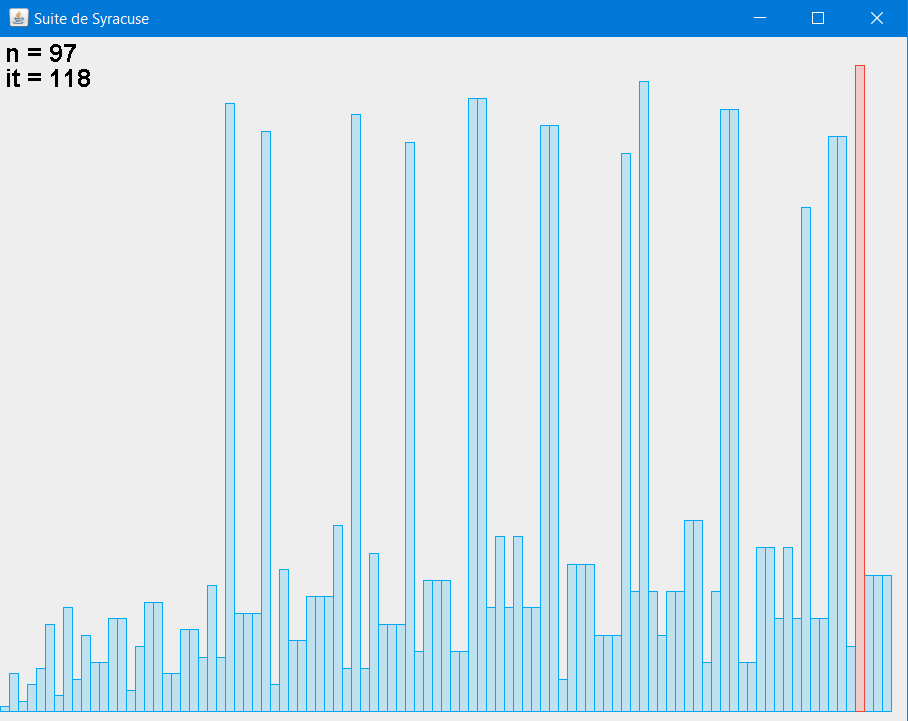
\includegraphics[scale=0.5]{images/syracuse_100.PNG}
\centering
\caption{Graphique de 2 à 100 en fonction de leur nombre d'itérations}
\label{syra100}
\end{figure}

La seconde interface porte sur les variations lors du calcul d'un nombre donné dans la suite de Syracuse. On peut passer la souris sur le graphique et il nous dit à quelle itération on est et la valeur actuelle (sur la Figure \ref{syra97}, on se trouve pendant la 84e itération avec une valeur de 9232).

\begin{figure}[H]
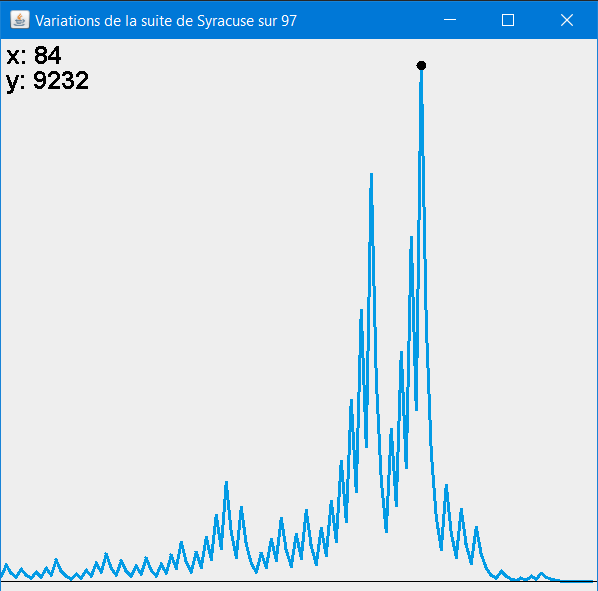
\includegraphics[scale=0.6]{images/syracuse_var_97.PNG}
\centering
\caption{Graphique sur de la variation dans la suite de Syracuse de 97}
\label{syra97}
\end{figure}

\subsubsection{Observations}

Pour la partie sur la comparaison du nombre d'itérations des différents nombres, on remarque que entre 2 et 100 (Figure \ref{syra100}), le nombre qui possède le plus grand nombre d'itérations est 97 avec 118 itérations. On remarque également qu'il y a plusieurs série de 2-3-5 nombres consécutifs qui ont le même nombre d'itérations, si on regarde entre 2 et 150, on a par exemple : 
\begin{itemize}
\item 12 et 13 avec 9 itérations
\item 28, 29 et 30 avec 18 itérations
\item 36, 37 et 38 avec 21 itérations
\item 44, 45 et 46 avec 16 itérations
\item 98, 99, 100, 101 et 102 avec 25 itérations
\item 130, 131, 132, 133 et 134 avec 28 itérations
\end{itemize}

Ensuite, sur les variations des nombres, on peur remarquer qu'on obtient des pics relativement importants sur des nombres qui ont un nombre important d'itérations. Pour 27, 31, 63, 73 et 97 (et probablement d'autres) on obtient la même valeur comme pic à 9232, comme si sur certains nombres on aurait une convergence vers une même fin qui commencerait à 9232.

\begin{figure}[H]
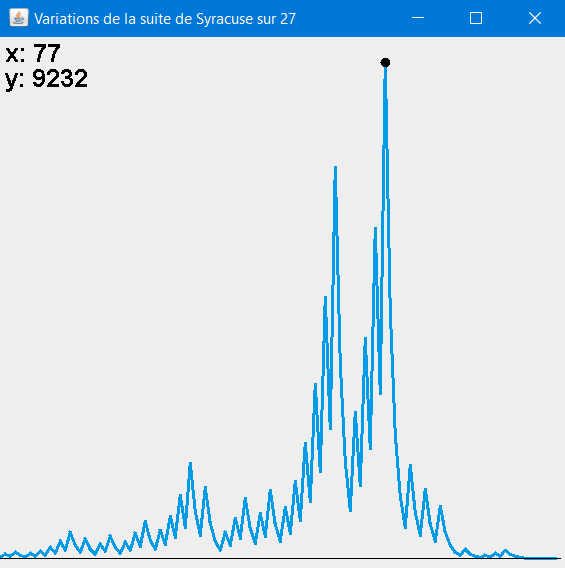
\includegraphics[scale=0.6]{images/syracuse_var_27.PNG}
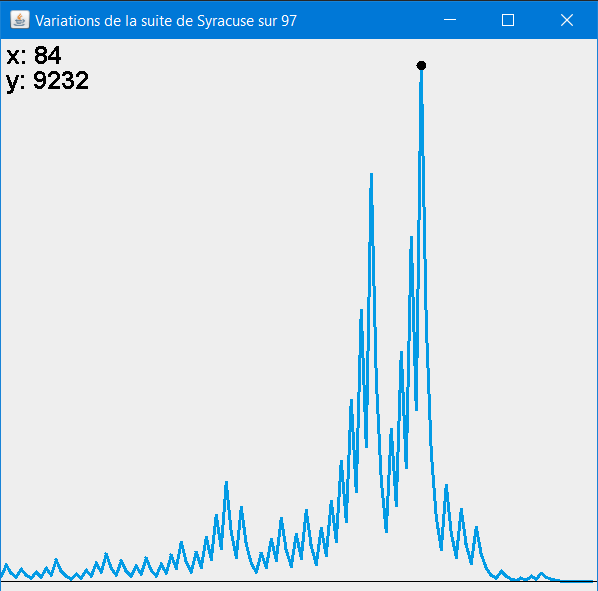
\includegraphics[scale=0.58]{images/syracuse_var_97.PNG}
\centering
\caption{Graphique sur de la variation dans la suite de Syracuse de 27 et 97}
\end{figure}

Les nombres qui ont la même fin de variations sont faciles à distinguer, ce sont tous les pics avec un écart plus important que la moyenne. Sur la figure \ref{pics}, toutes les valeurs étant au-dessus de la ligne rouge ont la même fin de variations commençant par 9232. Les nombres en dessous de la ligne rouge ont tous des variations tombantes comme celle de la Figure \ref{syra78} pour 68 et 78.

\begin{figure}[H]
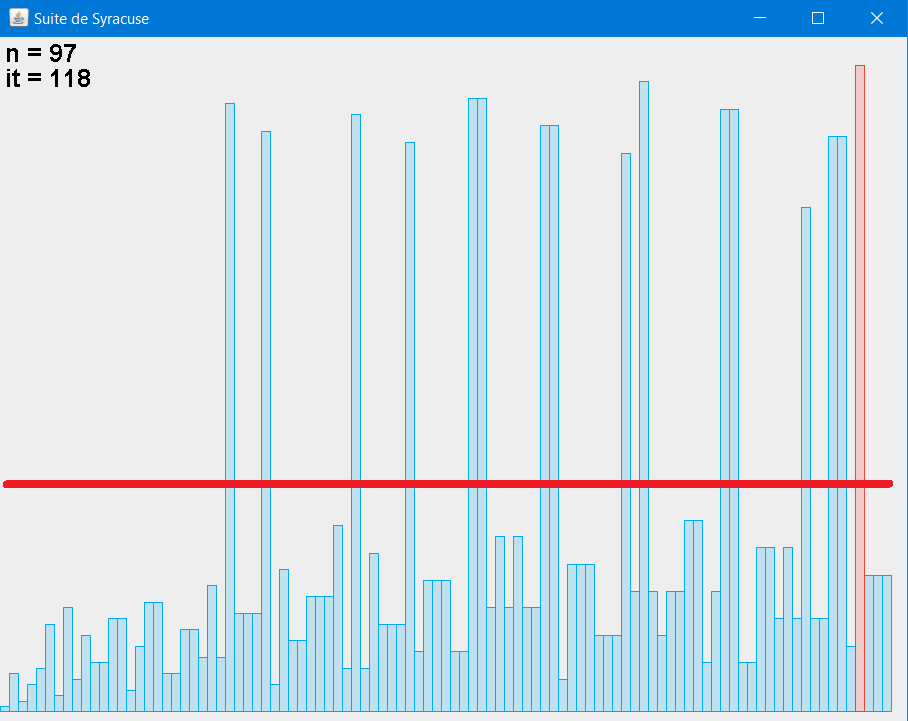
\includegraphics[scale=0.5]{images/syracuse_pics.PNG}
\centering
\caption{Graphique mettant en évidence les pics entre 2 et 100}
\label{pics}
\end{figure}

\begin{figure}[H]
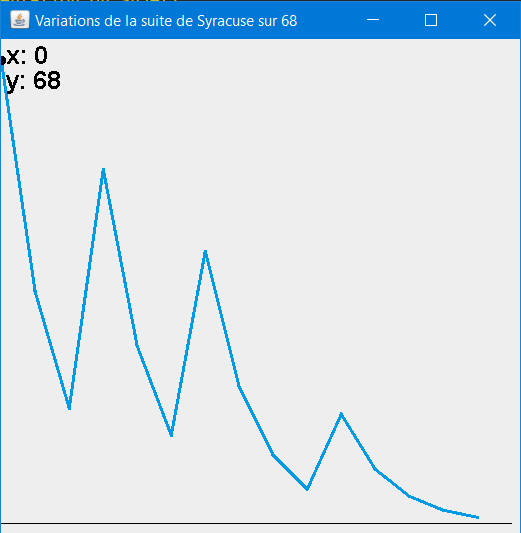
\includegraphics[scale=0.59]{images/syracuse_var_68.PNG}
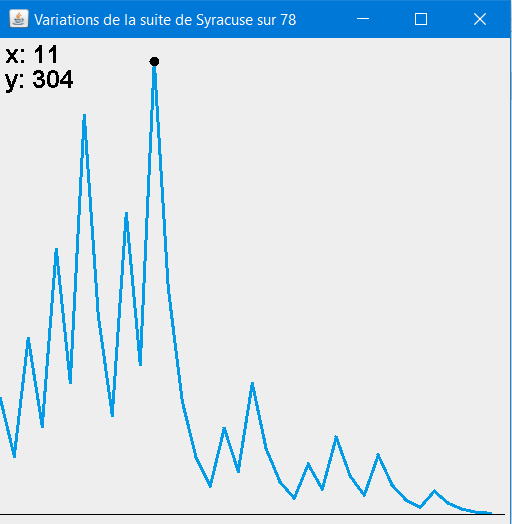
\includegraphics[scale=0.6]{images/syracuse_var_78.PNG}
\centering
\caption{Graphique sur la variation dans la suite de Syracuse de 68 et 78}
\label{syra78}
\end{figure}

\subsubsection{Test avec 5n+1}
Nous avons essayé d'utiliser la suite 5n+1 au lieu de 3n+1 ; seulement nous n'avons pas pu utiliser nos graphiques comme pour la suite 3n+1 car dans la suite il y a des valeurs pour lesquelles on se retrouve dans un cycle par exemple pour 5 on a un cycle 26, 13, 66, 33, 166, 83, 416, 208, 104, 52, 26, 13 ...\\
On obtient une suite qui a tendance a diverger si on prend par exemple 7. Si on prend 13 on retombe sur le cycle généré par 5 : 66, 33, 166, 83, 416, 208, 104, 52, 26, 13 ...




